\documentclass[11pt,a4paper]{article}
\usepackage{fontspec}
\setmainfont{TeXGyrePagella}
\usepackage[french]{babel}
\usepackage{graphicx,tikz,xcolor,geometry}
\usetikzlibrary{calc}
\geometry{margin=0pt}
\pagestyle{empty}
\definecolor{bleufonce}{HTML}{1B3A6B}
\definecolor{bleugris}{HTML}{5C7190}
\newcommand{\pos}[4]{\node[anchor=north west,inner sep=0pt,outer sep=0pt,text width=#3,align=left] at ($(current page.north west)+(#1,-#2)$) {#4};}
\newcommand{\sect}[1]{{\color{bleufonce}\bfseries\fontsize{17}{19}\selectfont #1}}
\newcommand{\bodyfont}{\fontsize{10.5}{13.2}\selectfont}
\newcommand{\smallfont}{\fontsize{9.5}{11.7}\selectfont}
\begin{document}
\begin{tikzpicture}[remember picture,overlay]
\draw[bleufonce,line width=.95pt,rounded corners=8mm]
  ($(current page.north west)+(5mm,-5mm)$) rectangle
  ($(current page.south east)+(-5mm,5mm)$);

\pos{10mm}{13mm}{189mm}{\sect{1. Découvrir Proteus}}
\pos{10mm}{25mm}{187mm}{{\bodyfont \textbf{Proteus} est un logiciel de conception et de simulation électronique. Son éditeur \textbf{ISIS} permet de placer des composants, de tracer leurs connexions et de tester le fonctionnement d'un circuit avant sa réalisation.}}
\pos{10mm}{44mm}{188mm}{\sect{À quoi sert Proteus ?}}
\pos{14mm}{56mm}{182mm}{{\bodyfont
  \textcolor{bleufonce}{\textbullet}\enspace \textbf{Dessiner :} construire un schéma électrique à l'aide de symboles.\\[1.1mm]
  \textcolor{bleufonce}{\textbullet}\enspace \textbf{Simuler :} vérifier le comportement d'un circuit sur ordinateur.\\[1.1mm]
  \textcolor{bleufonce}{\textbullet}\enspace \textbf{Observer :} examiner le résultat et rechercher les erreurs éventuelles.
}}

\node[anchor=north west,inner sep=0pt,outer sep=0pt] at ($(current page.north west)+(12mm,-87mm)$) {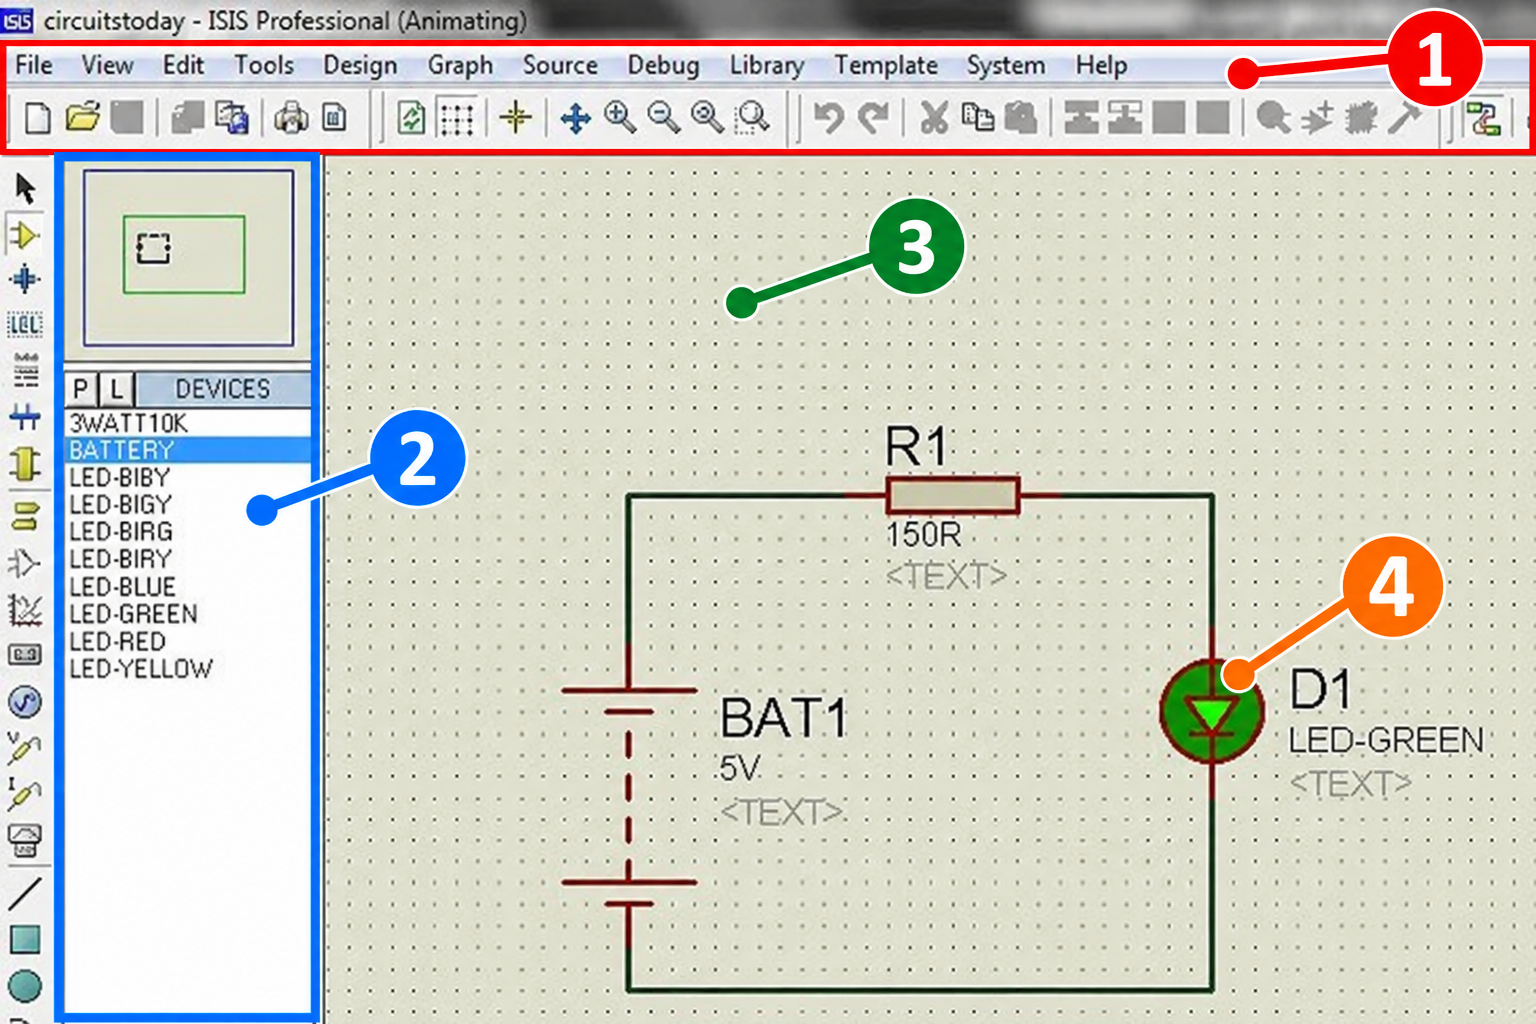
\includegraphics[width=186mm]{proteus_isis_circuit_tutorial_diagram.png}};
\pos{13mm}{213mm}{184mm}{{\color{bleugris}\fontsize{8.5}{10.3}\selectfont Figure 1 --- Interface de Proteus ISIS : les quatre repères désignent les zones à connaître.}}
\pos{14mm}{223mm}{85mm}{{\smallfont \textcolor{bleufonce}{\textbf{1. Barre de menus et d'outils :}} ouvrir un fichier et choisir les principales commandes.}}
\pos{109mm}{223mm}{85mm}{{\smallfont \textcolor{bleufonce}{\textbf{2. Bibliothèque des composants :}} rechercher et sélectionner une batterie ou une LED.}}
\pos{14mm}{237mm}{85mm}{{\smallfont \textcolor{bleufonce}{\textbf{3. Feuille de schéma :}} espace de placement et de connexion des composants.}}
\pos{109mm}{237mm}{85mm}{{\smallfont \textcolor{bleufonce}{\textbf{4. Circuit réalisé :}} exemple de batterie, résistance et LED en série.}}

\draw[bleufonce,line width=.65pt,rounded corners=2mm]
  ($(current page.north west)+(10mm,-253mm)$) rectangle
  ($(current page.north west)+(200mm,-261mm)$);
\pos{15mm}{255mm}{180mm}{{\fontsize{9.1}{10.4}\selectfont \textcolor{bleufonce}{\bfseries À retenir :} repérer la bibliothèque, la feuille de schéma et les outils avant de créer son montage.}}

\draw[bleufonce!55,line width=.45pt] ($(current page.south west)+(10mm,14.7mm)$) --
  ($(current page.south east)+(-10mm,14.7mm)$);
\node[anchor=south west,inner sep=0pt,text=bleufonce!80] at ($(current page.south west)+(10mm,7.4mm)$)
  {\fontsize{9.5}{11}\selectfont 2026/2027};
\node[anchor=south east,inner sep=0pt,text=bleufonce!80] at ($(current page.south east)+(-10mm,7.4mm)$)
  {\fontsize{9.5}{11}\selectfont Page 2};
\end{tikzpicture}
\null
\end{document}
